%!TEX root = mb.tex


%\section{Building block: Range match}
%An important operation over an encrypted packet is to determine if an encrypted field in the packet falls in an encrypted range.
%We will use the firewall as an example. 
%Consider the following firewall rule:
%
%Constructing an encryption scheme that allows checking if an encrypted value is in an encrypted range, has been a challenge in the applied cryptography community. The reason is that ..
%
%\begin{itemize}
%\item preserve the order between Encryptd values
%\item candidate: OPE
%\item candidate: mOPE
%\item So none of the existing schemes are satisfactory. A new scheme \RM.
%\end{itemize}
%
%\RM applies to cases when we know an upper bound on the values encrypted with OPE and this is a small number of values (say, less than 10,000).
%
%The small number of values permits us to improve in two ways over mOPE [1]
%No more interaction. We store the tree in mOPE on the gateway (client) side, which means that the gateway can compute a new encryption by itself without help from service provider. The storage at the gateway will remain small.
%Rare updates to ciphertexts. We can space out the ciphertexts of the values encrypted sufficiently. 
%
%This also enjoys a stronger security than OPE! It leaks less than order.
%The reason is that, the server does not learn the order between the values in packets, and only whether they map between two values in the rules. 
%
%this one is new
%
%discuss 
%
%would be good to explain the challenge from the 
%
%\todo{a more interesting name to the scheme}
%
%prefix gets mapped into interval, at most a certain number
%
%talk about building certain data structures that all works the same
%
%firewall need not change 

\subsection{Range match } \label{sec:range}




Many middleboxes perform detection over a {\it range} of port numbers or IP addresses. For example, a network administrator might wish to block access to all servers hosted by MIT, in which case the administrator would block access to the network prefix 18.0.0.0/8, \ie{}, 18.0.0.0-18.255.255.255. RangeMatch enables a middlebox to tell whether or not an IP address $v$ lines in between such a range $[s_1, e_1]$, where $s_1$ = 18.0.0.0 and $e_1$ = 18.255.255.255; however, the middlebox does not learn the values of $v$, $s_1$, or $e_1$.

%
The functionality of the RangeMatch scheme is to encrypt a set of ranges $[s_1, e_1]$, $\dots$, $[s_n, e_n]$ into  $[\Enc(s_1)$, $\Enc(e_1)]$, $\dots$, $[\Enc(s_n)$,  $\Enc(e_n)]$, and a value $v$ into $\Enc(v)$, such that anyone with access to these encryptions can determine in which range $v$ lies, while not learning the values of $s_1$, $e_1$, $\dots$, $s_n$, $e_n$, and $v$. 
For concreteness, we explain our scheme by considering $v$, $e_i$ and $s_i$ as IP addresses (although it can be used for encrypting ports too).

\noindent\textbf{Requirements.}
%
In order for this encryption scheme to fit \sys efficiently and securely, it must:

\begin{CompactEnumerate}[leftmargin=*]

\item  {\em be fast}: the throughput of encryption should be not much lower than network throughput. In particular, the scheme should preserve the ability to use {\em existing fast packet matching algorithms}, such as  various kinds of tries, area-based quadtrees, FIS-trees, or hardware-based algorithms~\cite{packet_classif}.  All of these rely on the ability of SP  to compute ``>'' between $v$ and the endpoints of an interval,
hence the encryption scheme should preserve this property. 




\item {\em provide strong security}: The encryption scheme should not leak $v$, $e_1$, $s_1$, $\dots$, $e_n$, $s_n$ to SP.
Ideally, SP does not learn anything about $v$ other than what interval it matches to. In  particular, even if $v_1$ and $v_2$ match the same range, SP should not learn their order. SP is allowed to learn the order relation of the intervals (in fact, in many setups, SP provides the intervals). \label{req:sec}


\item {\em be deterministic}: To integrate with NAT and to enable middleboxes to piece together packets from the same flow, each value should get  consistently  the same encryption. Any changes in the encryption assigned should happen rarely.  \label{req:injective}

\item {\em be format-preserving}: The encryption should have the same format as the data. Concretely, an encrypted IP address should look like an IP address.  This property is important to avoid changing the packet header structure, which would be a hurdle to adoption. 
 \end{CompactEnumerate}


Unfortunately, there is no encryption scheme that supports all these requirements. The closest schemes to these requirements  is {\em order-preserving encryption}, BCLO~\cite{boldyreva:ope} and mOPE~\cite{popa:mope}. However, these schemes are both significantly less secure and less efficient than our scheme. In terms of security, they leak the order between any two IP addresses encrypted, and not just whether they match the same interval or not. Moreover, BCLO~\cite{boldyreva:ope} leaks the top half of the bits too. In terms of performance, they cannot keep up with packet-processing demands, as they take milliseconds per encryption (as demonstrated in \S\ref{sec:eval}), which would only allow the gateway to forward a few hundred packets per second. 


Instead, we designed a new encryption scheme that satisfies all the requirements above called {\em range match} scheme. 
%The scheme takes advantage of the network setting; it does not rely on advanced cryptography%, so it can be easily understood and validated by a non-cryptographically trained reader. 
%Kay sez patronizing. I don't think so, but, it certainly is unnecessary and we are short on space!!!

\subsubsection{Our RangeMatch scheme} 



%We explain the scheme based on encryption IP addresses for a firewall and source IP addresses in packets, although the scheme is used in encryption other fields too, as explained in Sec.~\ref{xx}.

To encrypt the endpoints of the intervals, we sort them, and choose as their encryptions values equally distributed in the domain space in a way that preserves the order of the endpoints. For example, the encryption of the intervals 127.0.0.0/8 and 172.16.0.0/16, is [51.0.0.0, 102.0.0.0] and [153.0.0.0, 204.0.0.0]. This preserves the order of the intervals but does not leak anything else.

For now, consider that the gateway  maintains a mapping of each interval endpoint  to its encryption, called the {\em interval map}.  The interval map also contains the points $- \infty$ and $+ \infty$, encrypted with 0.0.0.0 and 255.255.255.255. 


When the gateway needs to encrypt an IP address $v$, the gateway first determines what  is the interval  $v$ falls in (we discuss below what happens when more than one interval matches). It uses the interval map to determine the encryptions of the endpoints of this interval. Then, to encrypt $v$, it chooses a random value in this interval.
For example, if $v$ is 127.0.0.1, a possible encryption is 48.124.24.85. This is great for security because the encryption does not retain any information about $v$ other than the range it is in. In particular, for two values $v_1$ and $v_2$ that match the same interval, SP does not learn their order. Thus, this satisfies the security requirement above, and makes our scheme more secure than order-preserving encryption schemes.

We need to specify how to encrypt $v$ when $v$ fits in multiple intervals or in no interval at all. Consider an example in which $v$ fits in no interval at all. Let $v$ be $127.0.0.0$ and the intervals be 18.0.0.0/8 and 172.16.0.0/16 with encryptions [51.0.0.0, 102.0.0.0] and [153.0.0.0, 204.0.0.0]. The encryption of $v$ should not be chosen at random between  102.0.0.0 and 153.0.0.0 because SP learns that $v$ is between the two intervals. Recall that we want SP  to learn only whether $v$ matches an interval or not, but nothing else. Hence, $v$ should be mapped to a random value anywhere in the intervals [0, 51.0.0.0), (102.0.0.0, 153.0.0.0) and (204.0.0.0, 255.255.255.255]. 

To achieve the desired security, the idea is to find the interval $I$ inside which $v$ should be mapped at random. The equation for $I$ is as follows. Consider the intervals {\em inside} which $v$ falls, and let $I_0, I_1, \dots, I_{n_I}$ be their encryptions. We always include the total interval $I_0 = [0,0,0,0, 255.255.255.255]$. Now consider the intervals {\em outside} of which $v$ falls and let $O_1, \dots, O_{n_O}$ be their encryptions. Then, to provide our desired security goal, $v$ should be chosen at random from the interval  
\begin{equation}
 I = I_0 \cap I_1 \cap ... \cap I_{n_I} - (O_1 \cup \dots \cup O_2). \label{eq:randominterval}
 \end{equation}

 


To satisfy requirement~\ref{req:injective}, we need to generate the random encryptions using a deterministic function. For this, we use a pseudorandom function~\cite{GoldreichVol1}, $\prf$, seeded in $k$.   Let $|I|$ be the size of the interval $I$. 
Then, the encryption of $v$ is the $\mathsf{index}$-th element in $I$, where $\mathsf{index}$ is 
\[ \mathsf{index}(v) = \prf_k(v)\ \mod\ |I|. \] 
  Note that, in the system's setup with two gateways, the gateways generate the same encryption because they share $k$. 

When encrypting IP addresses, we do not want two different IP addresses to map to the same encryption (which would break the NAT). Fortunately, the probability that two IP addresses get assigned to the same encryption is negligibly low for IPv6. This probability is very low for IPv4, but not low enough that a collision will not happen in a large interval of time. The reason is that each interval of encryptions is large because we distributed the endpoint encryptions evenly and because there is a small number of such endpoints in a realistic setting (e.g., a firewall has less than 100,000 rules). Suppose we have $n$ distinct rules, $m$ flows and a $w$-bit space, the probability of getting collision is approximately $1-e^\frac{-m^2 (n+1)}{2^{w+1}}$. Therefore, if $w=128$ (which is the case when we use IPv6), the probability is negligible in a normal setting. 

The last issue to address is addition and removal of intervals. For example, this can happen when a new rule is added to a firewall. 
Since we tried to spread out the encryptions of the intervals evenly in the IP space, there is no room for the new interval. We can 
readjust all the encryptions of these intervals to make space for the new interval. However, this would require the firewall hardware to reconfigure fully which is slow. Ideally, we would only reconfigure the firewall hardware incrementally, for the new interval. For this, we build on the idea from mOPE~\cite{popa:mope} and store the intervals at the gateway in a balanced scapegoat tree as in Fig.~\ref{fig:tree}. This tree is a search tree that has the property that when inserting or deleting a node, the number of other nodes that change encryption is small, namely, $O(\log n)$ amortized worst case where $n$ is the number of nodes. Each node in the tree is now encrypted similarly to before: the root gets the middle of the IP range,  the left node gets the middle of the IP space to the left of the middle, and so on, as in Fig.~\ref{fig:tree}.  Note that, since the tree is balanced, it maintains our desire of having the encryptions of endpoints roughly uniformly distributed.

\begin{figure}
  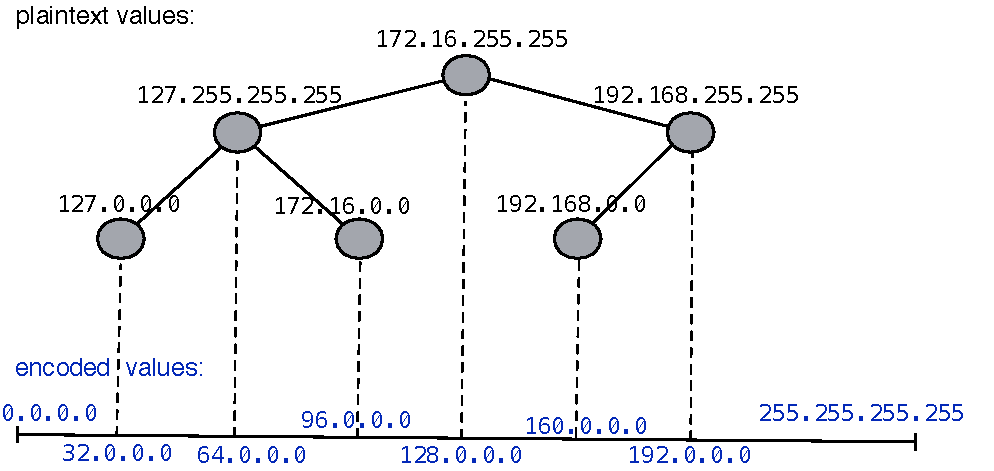
\includegraphics[width=3.45in]{fig/tree}
  \caption{\label{fig:tree} Range match tree. The values of nodes in the tree are the unencrypted IP addresses, and the blue values on the horizontal axis are their encryptions. }
\end{figure}



%We now explain concretely the API and the implementation of the scheme. 

\subsubsection{Gateway API and implementation}\label{s:rangealg}

\noindent\textbf{Gateway state.} The gateway keeps a small amount of state (in our implementation, about 200 bytes/range) encryption the intervals, but maintains no state per IP address encrypted or per connection. The gateway stores the tree in Fig.~\ref{fig:tree}: for each node, it stores the unencrypted endpoint, whether it is the left or  right margin of an interval, and the other endpoint of the interval it is part of. It does not need to store the encryption of the endpoint because this is easy to derive from the position in the tree. 


The gateway can use the following functions. EncryptRanges encrypts the initial ranges. Note that some ranges could consist of
one point only, namely $s = e$. 

% TO CUT TO REDUCE: put all these algorithms into one box
% framed takes space around it, above it, below it 

\begin{framed}
\begin{algorithmic}[1]

\Procedure{EncryptRanges}{[$s_1$, $e_1$], $\dots$, [$s_n$, $e_n$]}
  \State Build scapegoat tree on the values 
              $\{s_1, \dots, s_n\}$ 
              $\cup$ $\{e_1, \dots, e_n\}$ 
              $\cup$ $\{-\infty, \infty\}$.
  \State Assign an encryption $\enc(x)$ to each node $x$ in the tree:
  \begin{itemize}
  \item the root gets the middle of the IP range, $e$, 
  \item the node to the left of the root gets the middle of the interval to the left of $e$: ($e/2$),
  \item the right node gets the middle of the range
  to the right of $e$: ($3e/2$), and so on.
  \end{itemize}

  \State \Return{[$\enc(s_1)$, $\enc(e_1)$], $\dots$, [$\enc(s_n)$, $\enc(e_n)$]}
\EndProcedure

\end{algorithmic}
\end{framed}



EncryptValue encrypts the values to be matched against ranges.

\begin{framed}
\begin{algorithmic}[1]

\Procedure{EncryptValue}{$v$}
  \State Search the tree for $v$ to compute efficiently I as in Eq.~\ref{eq:randominterval}.
  \State Compute $\mathsf{index}(v) = \prf_k(v)\ \mod\ |I|.$ 
  \State Let $\enc(v)$ to be the $\mathsf{index}$-th element of $I$. 
  \State \Return $\left(\enc(v), \IV, \aes_k(\IV, v)\right)$ for random $\IV$. 
\EndProcedure

\end{algorithmic}
\end{framed}

Here is how to compute $I$ efficiently. When searching for $v$ in the tree, the gateway
can identify the tightest enclosing interval [$p_1$, $p_2$] in logarithmic time. 
 If $[p_1, p_2]$ are endpoints of the
same interval, then I = [$p_1$, $p_2$]. Otherwise, move towards the left in the tree until you identify the first endpoint
$\ell_1$
that belongs to an interval $[\ell_1, \ell_2]$ enclosing $v$. Then, using the tree, scan $[\ell_1, \ell_2]$ and eliminate
any intervals not containing $v$. The gateway can precompute and store this interval for every two consecutive nodes in the tree.

EncryptValue returns an AES encryption of $v$ too, because $\enc(v)$ is not decryptable. 

We now describe the procedure for AddRange and DeleteRange which add or delete an interval. 
These will modify the state at the gateway. Besides the interval added or deleted, a small number
of other intervals may be moved. For these, the algorithm returns the old and new encryption of the interval. 


\begin{framed}
\begin{algorithmic}[1]

\Procedure{AddRange}{$[s, e]$}
  \State Insert $s$ and $e$ into the scapegoat tree. If $s=e$, insert the value only once.
  %	
  \State Initialize $L$ to be the empty list.
  \If{tree needs to be rebalanced}
  	\State Record which nodes change position in the tree during rebalancing, together with 
	their old and new encryptions. Namely, record	\[L = \{ \en_1 \leftarrow \en^*_1, \dots, \en_m \rightarrow \en^*_m\},\] where $m$ is the number of nodes who changed position in the tree, and $\en_i$ and $\en^*_i$ are the old and new encryption of the $i$-th node that changed position. 
  \EndIf
  \State Compute  $\enc(s)$ and $\enc(e)$, the encryptions of $s$ and $e$, as in EncryptRanges.
   \State \Return{$[\enc(s), \enc(e)], L$}
\EndProcedure

\end{algorithmic}
\end{framed}

%  \State Determing the smallest and the largest encryption in the values $[\enc(s), \enc(e)]$ and $L$, and call this $\dirtyrange$.

Since we are using a scapegoat tree, the number of nodes that change position during rebalancing is amortized worst case $O(\log n)$ where $n$ is the total number of nodes in the scapegoat tree. 

A natural question is whether there exists a scheme that does not need to adjust already encrypted intervals. For a related setting, Popa et al.~\cite{popa:mope} proved that whenever one supports ``>'' over  encrypted data, there must be some adjustment similar to this; the proof holds for our setting too.  

DeleteRange is similar, except that the result contains only $L$. 

\subsubsection{Cloud API}

The cloud can run ``$\ge$'' and "$\le$" between any encrypted value $\enc(v)$ and an encrypted endpoint $\enc(s)$ and $\enc(e)$, and will obtain a correct answer. Computing $\enc(v_1) < \enc(v_2)$  between two encrypted values in the same range is meaningless, and returns a random value.


\subsubsection{Security guarantees}

The scheme achieves our desired security goal: the only information leaked about a value $v$ encrypted is which ranges it matches. 
In particular, the scheme is not order preserving because it does not leak the order of two encrypted values that match the same range. It is easy to check that the scheme is secure: since the encryption of $v$ is random in $I$ (Eq.~\ref{eq:randominterval}), the scheme only leaks the fact that $v$ is in $I$. $I$ is chosen in such a way that the only information about $v$ it encodes is which intervals $v$ matches and which it does not match.




% PROTOCOL

% the gateway encrypts teh IP has to be clear

% Here somewhere we need to discuss that there is one encryption scheme adn then there is how we use it for ports and other ip addresses.

% in the firewall protocol describe how hardware does not change 

% can use the same processing 
